% Options for packages loaded elsewhere
\PassOptionsToPackage{unicode}{hyperref}
\PassOptionsToPackage{hyphens}{url}
%
\documentclass[
]{article}
\usepackage{amsmath,amssymb}
\usepackage{iftex}
\ifPDFTeX
  \usepackage[T1]{fontenc}
  \usepackage[utf8]{inputenc}
  \usepackage{textcomp} % provide euro and other symbols
\else % if luatex or xetex
  \usepackage{unicode-math} % this also loads fontspec
  \defaultfontfeatures{Scale=MatchLowercase}
  \defaultfontfeatures[\rmfamily]{Ligatures=TeX,Scale=1}
\fi
\usepackage{lmodern}
\ifPDFTeX\else
  % xetex/luatex font selection
\fi
% Use upquote if available, for straight quotes in verbatim environments
\IfFileExists{upquote.sty}{\usepackage{upquote}}{}
\IfFileExists{microtype.sty}{% use microtype if available
  \usepackage[]{microtype}
  \UseMicrotypeSet[protrusion]{basicmath} % disable protrusion for tt fonts
}{}
\makeatletter
\@ifundefined{KOMAClassName}{% if non-KOMA class
  \IfFileExists{parskip.sty}{%
    \usepackage{parskip}
  }{% else
    \setlength{\parindent}{0pt}
    \setlength{\parskip}{6pt plus 2pt minus 1pt}}
}{% if KOMA class
  \KOMAoptions{parskip=half}}
\makeatother
\usepackage{xcolor}
\usepackage[margin=1in]{geometry}
\usepackage{graphicx}
\makeatletter
\def\maxwidth{\ifdim\Gin@nat@width>\linewidth\linewidth\else\Gin@nat@width\fi}
\def\maxheight{\ifdim\Gin@nat@height>\textheight\textheight\else\Gin@nat@height\fi}
\makeatother
% Scale images if necessary, so that they will not overflow the page
% margins by default, and it is still possible to overwrite the defaults
% using explicit options in \includegraphics[width, height, ...]{}
\setkeys{Gin}{width=\maxwidth,height=\maxheight,keepaspectratio}
% Set default figure placement to htbp
\makeatletter
\def\fps@figure{htbp}
\makeatother
\setlength{\emergencystretch}{3em} % prevent overfull lines
\providecommand{\tightlist}{%
  \setlength{\itemsep}{0pt}\setlength{\parskip}{0pt}}
\setcounter{secnumdepth}{-\maxdimen} % remove section numbering
\usepackage{titlesec}
\titleformat*{\section}{\normalfont\Large\bfseries\flushleft}
\titleformat*{\subsection}{\normalfont\large\bfseries\flushleft}
\titleformat*{\subsubsection}{\normalfont\normalsize\bfseries\flushleft}
\usepackage{amsmath}
\newcommand*{\defeq}{\mathrel{\vcenter{\baselineskip0.5ex \lineskiplimit0pt \hbox{\scriptsize.}\hbox{\scriptsize.}}}=}
\newcommand*{\eqdef}{=\mathrel{\vcenter{\baselineskip0.5ex \lineskiplimit0pt \hbox{\scriptsize.}\hbox{\scriptsize.}}}}
\ifLuaTeX
  \usepackage{selnolig}  % disable illegal ligatures
\fi
\usepackage{bookmark}
\IfFileExists{xurl.sty}{\usepackage{xurl}}{} % add URL line breaks if available
\urlstyle{same}
\hypersetup{
  pdftitle={Statistical Learning (5454) - Assignment 4},
  pdfauthor={Matthias Hochholzer, Lukas Pirnbacher, Anne Valder},
  hidelinks,
  pdfcreator={LaTeX via pandoc}}

\title{Statistical Learning (5454) - Assignment 4}
\author{Matthias Hochholzer, Lukas Pirnbacher, Anne Valder}
\date{Due: 2024-06-10}

\begin{document}
\maketitle

\section{Exercise 1}\label{exercise-1}

We generate data from the additive error model
\(Y = f(X_1,X_2) + \epsilon\), where \(f(X_1, X_2)\) is a sum of
sigmoids, i.e.
\[ f(X_1,X_2) = \sigma(a_1^\top X_1) + \sigma(a_2^\top X_2), \] with
\(a_1 = (3, 3)'\), \(a_2 = (3,-3)'\) and bivariate standard Gaussian
variables \(X_j\), \(j = 1, 2\). The variance of the independent
Gaussian error \(\epsilon\) is chosen such that the signal-to-noise
ratio as measured by the respective variances equals four. We generate a
training set of size 100 and a test sample of size 10,000.

We then fit neural networks with weight decay of 0.0005 and vary the
number of hidden units from 0 to 10. We record the average test error
\[\mathbb{E}_{\text{Test}}(Y - \hat{f}(X_1,X_2))^2\] for each of 10
random starting weights.

\begin{verbatim}
##    hidden_units mean_test_error sd_test_error
## 1             0       0.1569335   0.009344669
## 2             1       0.1805459   0.031403812
## 3             2       0.1531848   0.031377711
## 4             3       0.1357561   0.007124503
## 5             4       0.1354813   0.005213214
## 6             5       0.1347336   0.005268805
## 7             6       0.1309809   0.003254704
## 8             7       0.1306211   0.005273894
## 9             8       0.1320959   0.005098204
## 10            9       0.1333377   0.006381811
## 11           10       0.1320844   0.005652836
\end{verbatim}

Let us now visualize the results and interpret them.

\includegraphics{A4_files/figure-latex/unnamed-chunk-5-1.pdf}

Out of all the models under consideration, the neural network with a
single hidden unit performs worst. It has the largest mean average test
error and also the largest variation in the average test error for
different random starting weights. Somewhat surprisingly, the linear
model, i.e.~the neural network with no hidden units, performs almost as
good as the neural network with two hidden units. While the mean average
test errors of these two models are similar, the average test error is
much less sensitive to different starting weights in case of the linear
model. All neural networks with 3 or more hidden units have a similar
performance, both in terms of the mean average test error and the
standard deviation of the average test error for different random
starting weights. Overall, we conclude that choosing a larger number of
hidden units and imposing shrinkage via weight decay appears to be
better than having too few hidden units in the first place.

\newpage

\section{Exercise 2}\label{exercise-2}

The data sets \texttt{zip.train} and \texttt{zip.test} from package
\textbf{ElemStatLearn} contain information on the gray color values of
the pixels on a \(16 \times 16\) pixel image of hand-written digits. We
first visualize for each digit one randomly selected observation.

\includegraphics{A4_files/figure-latex/unnamed-chunk-7-1.pdf}

We now fit a multinomial logistic regression model to the training data
and evaluate it on the training and the test data. Before fitting the
model, however, we transform the data such that the regressors are
scaled on the unit interval.

We now determine the overall misclassification rate on the training and
the test data and the digit-specific misclassification rates on the test
data.

\begin{verbatim}
## [1] "misclassification rate (training data): 0.01%"
\end{verbatim}

\begin{verbatim}
## [1] "misclassification rate (test data): 12.11%"
\end{verbatim}

\begin{verbatim}
## [1] "digit-specific misclassification rates (test data):"
\end{verbatim}

\begin{verbatim}
##        0        1        2        3        4        5        6        7 
##   "3.9%"  "4.55%" "18.69%" "14.46%"    "21%" "16.88%"  "9.41%" "14.29%" 
##        8        9 
## "22.89%"  "6.78%"
\end{verbatim}

The misclassification rate on the training data is exceptionally low,
while the one on the test data is fairly high. The digits 8,4 and 2 are
particularly difficult to classify, whereas the model does a good job in
classifying 0,1, and 9.

The substantial discrepancy in performance between training and test
data suggests that overfitting may be an issue. Hence, we add a positive
weight decay of 0.05 when fitting the multinomial logistic regression
model in order to regularize it.

\begin{verbatim}
## [1] "misclassification rate (training data): 0.3%"
\end{verbatim}

\begin{verbatim}
## [1] "misclassification rate (test data): 9.32%"
\end{verbatim}

\begin{verbatim}
## [1] "digit-specific misclassification rates (test data):"
\end{verbatim}

\begin{verbatim}
##        0        1        2        3        4        5        6        7 
##   "3.9%"  "4.55%" "15.66%" "10.84%"  "13.5%" "13.75%"  "7.65%"  "10.2%" 
##        8        9 
## "15.06%"  "5.65%"
\end{verbatim}

Adding weight decay slightly increases the misclassification rate on the
training data, but reduces the misclassification rate on the test data.
The improved classification performance is particularly pronounced for
the ``difficult'' digits (8 and 4). Overall, adding a Ridge penalty to
the loss function, i.e.~adding the weight decay, improves the
out-of-sample performance of our model by mitigating the overfitting
problem.

\newpage

\section{Exercise 3}\label{exercise-3}

We continue using the data sets \texttt{zip.train} and \texttt{zip.test}
from package \textbf{ElemStatLearn}. However, we now only use a subset
of size 320 from \texttt{zip.train}, with an equal number of
observations for each digit to fit a multinomial logistic regression
model and a neural network. We use the remaining observations from
\texttt{zip.train} and the test data to evaluate the fitted models.

Given the small sample size of the training data, overfitting is most
likely an issue. We therefore visualize the performance on the test data
in dependence of the training epochs (\# epochs
\(\in \{10,20,30,50,100,150,200\}\)) when fitting the models.

\includegraphics[width=0.9\linewidth]{A4_files/figure-latex/unnamed-chunk-13-1}

\includegraphics[width=0.9\linewidth]{A4_files/figure-latex/unnamed-chunk-14-1}

\includegraphics[width=0.9\linewidth]{A4_files/figure-latex/unnamed-chunk-15-1}

\includegraphics[width=0.9\linewidth]{A4_files/figure-latex/unnamed-chunk-16-1}

The plots are in line with our assumption that overfitting is an issue
in this exercise. For all models (multinomial logit, neural networks
with 5, 10 and 20 hidden units) the misclassification rate on the test
data increases as the number of training epochs exceeds 30. Hence, in
the absence of a more explicit form of regularization (e.g.~a positive
weight decay) stopping the optimization routine early can be helpful to
improve out-of-sample performance.

\newpage

\section{Exercise 4}\label{exercise-4}

In the following we will estimate a predictive model for the
\texttt{Default} data from the \textbf{ISLR2} package. We fit a neural
network using a single hidden layer with 10 units and dropout
regularization.

\includegraphics{A4_files/figure-latex/unnamed-chunk-18-1.pdf}

The linear logistic regression model performs very well on the test data
and has a classification accuracy of 97.18\%. Our neural network also
performs well and has a slightly lower accuracy of 97.09\%. Looking at
the plots above, we can see that the value of the loss function
decreases as the number of training epochs increases - for both the
training and the test data. Given that the loss function evaluated at
the test data does not increase as the number of epochs grows larger, we
find no evidence for overfitting. The classification performance
slightly improves as the number of training epochs increases. However,
it does not improve monotonically and the marginal gains are rather
negligible.

We now compare the classification performance of the two models more
closely, by looking at their ROC curve and confusion matrix. In the ROC
plot we observe that the curves for the linear logistic regression model
and the neural network follow each other closely. The confusion
matrices, however, highlight some subtle differences between the two
models. The logistic regression model predicts almost twice as many
defaults (50 in total, 13 of them incorrectly) as the neural network (27
in total, 3 of them incorrectly).

\begin{verbatim}
## Setting levels: control = 0, case = 1
\end{verbatim}

\begin{verbatim}
## Setting direction: controls < cases
\end{verbatim}

\begin{verbatim}
## Setting levels: control = 0, case = 1
\end{verbatim}

\begin{verbatim}
## Setting direction: controls < cases
\end{verbatim}

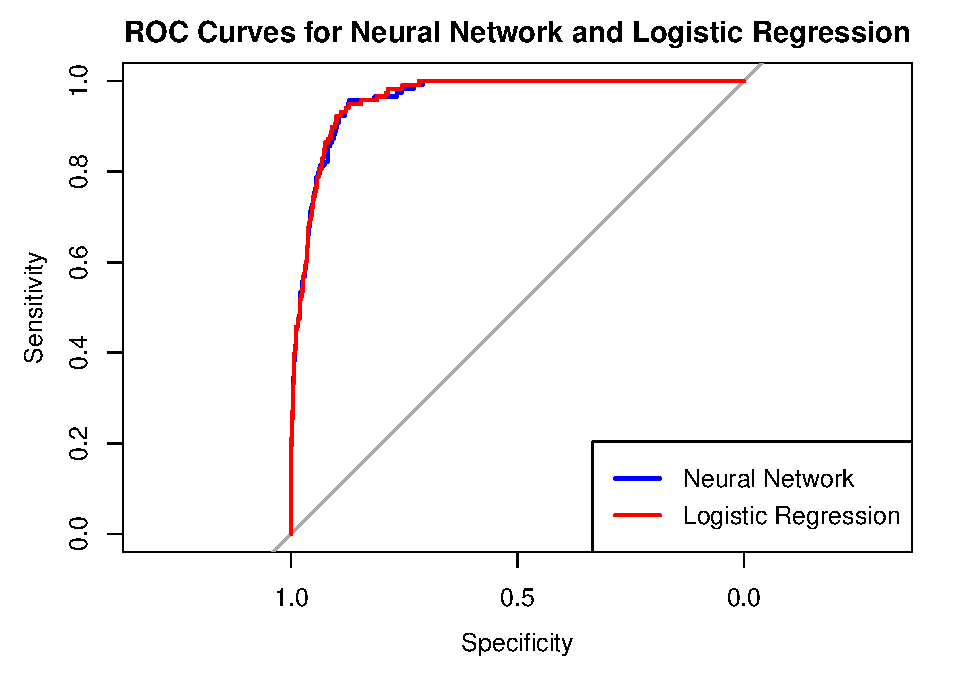
\includegraphics{A4_files/figure-latex/unnamed-chunk-19-1.pdf}

\begin{verbatim}
## AUC for Neural Network: 0.9611066
\end{verbatim}

\begin{verbatim}
## AUC for Logistic Regression: 0.9622321
\end{verbatim}

\begin{verbatim}
## [1] "Neural Network:"
\end{verbatim}

\begin{verbatim}
## Confusion Matrix and Statistics
## 
##           Reference
## Prediction    0    1
##          0 3212   94
##          1    3   24
##                                           
##                Accuracy : 0.9709          
##                  95% CI : (0.9646, 0.9763)
##     No Information Rate : 0.9646          
##     P-Value [Acc > NIR] : 0.02474         
##                                           
##                   Kappa : 0.3221          
##                                           
##  Mcnemar's Test P-Value : < 2e-16         
##                                           
##             Sensitivity : 0.9991          
##             Specificity : 0.2034          
##          Pos Pred Value : 0.9716          
##          Neg Pred Value : 0.8889          
##              Prevalence : 0.9646          
##          Detection Rate : 0.9637          
##    Detection Prevalence : 0.9919          
##       Balanced Accuracy : 0.6012          
##                                           
##        'Positive' Class : 0               
## 
\end{verbatim}

\begin{verbatim}
## [1] "Logistic Regression:"
\end{verbatim}

\begin{verbatim}
## Confusion Matrix and Statistics
## 
##           Reference
## Prediction    0    1
##          0 3202   81
##          1   13   37
##                                           
##                Accuracy : 0.9718          
##                  95% CI : (0.9656, 0.9772)
##     No Information Rate : 0.9646          
##     P-Value [Acc > NIR] : 0.01177         
##                                           
##                   Kappa : 0.4284          
##                                           
##  Mcnemar's Test P-Value : 4.829e-12       
##                                           
##             Sensitivity : 0.9960          
##             Specificity : 0.3136          
##          Pos Pred Value : 0.9753          
##          Neg Pred Value : 0.7400          
##              Prevalence : 0.9646          
##          Detection Rate : 0.9607          
##    Detection Prevalence : 0.9850          
##       Balanced Accuracy : 0.6548          
##                                           
##        'Positive' Class : 0               
## 
\end{verbatim}

\newpage

\section{Exercise 5}\label{exercise-5}

Now we perform document classification on the \texttt{IMDb} data set,
which is available as part of the \textbf{torchdatasets} package. We
limit the dictionary size to the 10,000 most frequently-used words and
tokens. Again, we use James et al.~(2021, Chapter 10 torch version). We
begin by loading the data and creating a \texttt{imdb\_tain} and
\texttt{imdb\_test} object. Each element of \texttt{imdb\_train} is a
vector of numbers between 1 and 10000 (the document), referring to the
words found in the dictionary. Next we write a function to one-hot
encode each document in a list of documents, and return a binary matrix
in sparse-matrix format. To construct the sparse matrix, one supplies
just the entries that are nonzero. In the last line we call the function
\texttt{sparseMatrix()} and supply the row indices corresponding to each
document and the column indices corresponding to the words in each
document, since we omit the values they are taken to be all ones. Words
that appear more than once in any given document still get recorded as a
one. Next we fit a fully-connected neural network with two hidden
layers, each with 16 units and ReLU activation.

After fitting the fully-connected neural network we can now look at the
results with the dictionary size 1000. We look at how the accuracy and
the loss of our train, test and validation set evolve over 10 epochs.
The accuracy graph displays that for the dictionary size of 1000 the
accuracy is highest for the validation set (above 0.88), followed by the
train set and lowest for the test set. Also for the train set the
accuracy increased sharply after the first 2 epochs. For test and train
it starts higher up but has higher variability. Considering the loss, we
see a similar development for our train set: For the first 2 epochs the
loss is rather high and then drops down and remains at more stable
level. The loss for the test and validation sets starts at a lower point
again, with the validation loss being below the test loss.

\includegraphics{A4_files/figure-latex/unnamed-chunk-21-1.pdf} We then
vary the dictionary size and try out values 500, 1000, 3000, 5000,
10,000 and consider the effects of this varying dictionary size. We
observe that the larger the dictionary size the higher the accuracy
(above 0.95 for dictionary size 10,000) and the lower the loss for the
training set. Moreover, the higher the accuracy of the training set, the
(slightly) higher the accuracy of the validation and test sets. In
addition, from the loss plots we can observe that the higher the
dictionary size, the more the loss varies between training, test and
validation set. Furthermore, the loss for the test set increases
strongly with more epochs, while the loss for the training data set
decreases (with more epochs).

\includegraphics{A4_files/figure-latex/unnamed-chunk-22-1.pdf}

\includegraphics{A4_files/figure-latex/unnamed-chunk-23-1.pdf}

\includegraphics{A4_files/figure-latex/unnamed-chunk-24-1.pdf}

\includegraphics{A4_files/figure-latex/unnamed-chunk-25-1.pdf}

\end{document}
